% Windows: протестировано для MikTeX+TeXworks в режиме pdfLatex.
%
% Linux:
% Для получения pdf используйте команду  pdflatex rfa_2021.tex.
% Команда latex rfa_2021.tex выведет сообщение об ошибке.
%
\NeedsTeXFormat{LaTeX2e}
\documentclass[10pt,a4paper]{book}
\usepackage{NumMet_2022}
%--- Здесь можно вставить необходимые стили ---
% \usepackage{...}
%
%--- Здесь можно добавить свои команды --------
% \newcommand{}
\newcommand{\ceq}{\mathrel{\vcenter{\hbox{:=}}}}
%----------------------------------------------
\selectlanguage{russian}
\begin{document}
%===========================  ШАПКА СТАТЬИ =================================
\Article{О реализации параллельного алгоритма глобальной оптимизации с использованием набора инструментов Intel oneAPI
}%Обновить перевод названия
    {On implementation of the parallel global optimization algorithm with the Intel oneAPI toolkit}
    
\Abstract{В статье рассматривается параллельный алгоритм решения задач глобальной оптимизации и обсуждается его реализация с использованием набора инструментов Intel oneAPI. Предполагается, что целевая функция задачи задана как <<черный ящик>> и удовлетворяет условию Липшица. Изложенный в статье параллельный алгоритм использует схему редукции размерности на основе кривых Пеано, которые непрерывно и однозначно отображают отрезок вещественной оси на гиперкуб.
В качестве средства для реализации параллельного алгоритма использован инструментарий Intel oneAPI, который позволяет писать один код как для центрального процессора, так и для графических ускорителей. Приведены результаты вычислительных экспериментов, полученные при решении серии сложных задач многоэкстремальной оптимизации.}
%обновить перевод - сейчас он для старой аннотации
    {The paper considers the parallel global optimization algorithm ans discusses its implementation with the Intel oneAPI toolkit. We suppose that the objective function is given as a black-box and satisfies the Lipschitz condition. The parallel algorithm presented in the paper uses the scheme of dimensionality reduction employing the Peano curve, which continuously maps an interval of the real axis onto a hypercube. The Intel OneApi tools, that allows one to write the same code for both the central processor and the graphics accelerator, were used for implementation of the parallel global optimization algorithm. The results of numerical experiments obtained by solving a series of time-consuming multiextremal optimization problems are presented.}

\Keywords{глобальная оптимизация,
многоэкстремальные функции,
параллельные вычисления,
редукция размерности,
графические ускорители,
Intel OneAPI.}
        {global optimization,
multiextremal functions,
parallel computing,
reduction of dimensionality,
graphics accelerators,
Intel OneApi.}

\Acknowledgements{Работа выполнена при поддержке программы Центра компетенций OneAPI в ННГУ, Министерства науки и высшего образования РФ (проект № 0729-2020-0055) и научно-образовательного математического центра «Математика технологий будущего» (проект № 075-02-2021-1394).}
    {Работа выполнена при поддержке программы Центра компетенций OneAPI в ННГУ, Министерства науки и высшего образования РФ (проект № 0729-2020-0055) и научно-образовательного математического центра «Математика технологий будущего» (проект № 075-02-2021-1394).}

\Citation{Баркалов К.А., Лебедев И.Г., Силенко Я.В.
    О реализации параллельного алгоритма глобальной оптимизации с использованием набора инструментов Intel oneAPI~//
    Вычислительные методы и программирование. 2022.
    \textbf{??}, \No~?. \pageref*{firstPage}--\pageref*{LastPage}.  
    doi 10.26089/NumMet.v??r???.}
    {K.~A.~Barkalov, I.~G.~Lebedev, Ya.~V.~Silenko,
    On implementation of the parallel global optimization algorithm with the Intel oneAPI toolkit
		``Numerical methods and programming,''
    Numerical Methods and Programming. \textbf{??} (?), 
    \pageref*{firstPage}--\pageref*{LastPage} (2022).
    doi~10.26089/NumMet.v??r???.}


\UDC{519.853.4}
\DOI{10.26089/NumMet.v??r???}% заполняет редакция
\VOL{??}{?}
\YEAR{2022}
\Received{16 октября 2022 г.}{October 16, 2022}
\Accepted{?? ??????? 2022 г.}{??????? ??, 2022}



\Author{К.~А.~Баркалов}{Konstantin~A.~Barkalov}
\FullName{Баркалов Константин Александрович}{Konstantin~A.~Barkalov}
% Место работы 1
\Institution{Нижегородский государственный университет им. Н.И. Лобачевского}
{Lobachevsky State University of Nizhny Novgorod}
\Address{пр. Гагарина, д. 23.}{Gagarin Ave., 23.}
\Postcode{603022}
\City{Нижний Новгород}{Nizhny Novgorod}
\CountryOfResidence{Российская Федерация}{Russia}
\AcademicDegree{
Доктор технических наук}{D.Sc.}
\Position{профессор}{professor}
\Orcid{0000-0001-5273-2471}
\Email{konstantin.barkalov@itmm.unn.ru}



\Author{И.~Г.~Лебедев}{Ilya~G.~Lebedev}
\FullName{Лебедев Илья Генадьевич}{Ilya~G.~Lebedev}
% Место работы 1
\Institution{Нижегородский государственный университет им. Н.И. Лобачевского}
{Lobachevsky State University of Nizhny Novgorod}
\Address{пр. Гагарина, д. 23.}{Gagarin Ave., 23.}
\Postcode{603022}
\City{Нижний Новгород}{Nizhny Novgorod}
\CountryOfResidence{Российская Федерация}{Russia}

\Position{заведующий лабораторией}{head of laboratory}
\Orcid{0000-0002-8736-0652}
\Email{ilya.lebedev@itmm.unn.ru}

\Author{Я.~В.~Силенко}{Yanina~V.~Silenko}
\FullName{Силенко Янина Вадимовна}{Yanina~V.~Silenko}
% Место работы 1
\Institution{Нижегородский государственный университет им. Н.И. Лобачевского}
{Lobachevsky State University of Nizhny Novgorod}
\Address{пр. Гагарина, д. 23.}{Gagarin Ave., 23.}
\Postcode{603022}
\City{Нижний Новгород}{Nizhny Novgorod}
\CountryOfResidence{Российская Федерация}{Russia}
\Position{лаборант}{laboratory assistant}
\Orcid{0000-0003-4894-2497}
\Email{yanina.silenko@itmm.unn.ru}

\MakeArticleHeader
%========================= КОНЕЦ ШАПКИ СТАТЬИ ==============================

\pagebreak



\section{Постановка задачи}

Задачи поиска минимума многоэкстремальных функций часто возникают в различных областях науки, таких как химия, физика и т.д. В частности, такие задачи возникают при разработке новых лекарственных препаратов [\ref{rfa:rulit:lit1}], при поиске конфигураций новых химических соединений [\ref{rfa:rulit:lit2},\ref{rfa:rulit:lit3}]. Задачи глобальной оптимизации возникают и во многих других приложениях [\ref{rfa:rulit:lit4}]. Традиционной сферой применения методов глобальной оптимизации стала идентификация параметров математических моделей по данным экспериментов. В задачах такого вида требуется провести поиск значений неизвестных параметров модели, при которых результаты расчетов близки к результатам, полученным экспериментально [\ref{rfa:rulit:lit5}].

Мы будем рассматривать задачу глобальной оптимизации в следующей постановке: требуется найти глобальный минимума$y^*$ функции $\varphi(y)$ в гиперинтервале $D$, т.е. 
\begin{equation}
\label{task}
\varphi(y^*)=\min\{\varphi(y):y\in D\}, \; D=\{y\in R^N:a_i\leq x_i\leq{b_i}, 1\leq{i}\leq{N}\}.
\end{equation}

Будем предполагать, что информация о структурных свойствах целевой функции $\varphi(y)$ неизвестна, а сама функция задается как <<черный ящик>>, т.е. с помощью некоторого реализованного программно алгоритма вычисления ее значений. Также будем предполагать, что $\varphi(y)$ удовлетворяет Липшица 
\begin{equation}
\label{lip}
|\varphi(y_1)-\varphi(y_2)|\leq L\Vert y_1-y_2\Vert,y_1,y_2\in D,0<L<\infty,
\end{equation}
причем константа Липшица $L$ априори неизвестна.

Многие известные алгоритмы липшицевой глобальной оптимизации основаны на идее редукции размерности и адаптации одномерных алгоритмов для решения многомерных задач [\ref{rfa:rulit:lit6},\ref{rfa:rulit:lit7}]. 
В данной работе мы будем использовать подход из [\ref{rfa:rulit:lit8}, \ref{rfa:rulit:lit9}], основанный на идее редукции размерности с помощью кривой Пеано  
$y(x)$, которая непрерывно и однозначно отображает отрезок вещественной оси $[0,1]$ на $N$-мерный гиперкуб:
\begin{equation}
\label{cube}
\lbrace y\in R^N:-2^{-1}\leq y_i\leq 2^{-1}, 1\leq i\leq N\rbrace=\{y(x): 0\leq x\leq 1\}.
\end{equation}
С использованием отображения $y(x)$ решение исходной задачи (\ref{task}) сводится к минимизации одномерной функции на отрезке $[0,1]$, т.е.
\begin{equation}
\label{oneDimTask}
\varphi(y^*)=\varphi(y(x^*))=\min\{\varphi(y(x)): x\in [0,1]\}.
\end{equation}
 
Указанный способ редукции размерности обладает следующим важным свойством: сохраняется ограниченность относительных разностей функции , т.е. если в области $D$ функция $\varphi(y)$ удовлетворяла условию Липшица, то на интервале $[0,1]$ функция $\varphi(y(x))$ будет удовлетворять равномерному условию Гельдера
\begin{equation}
\label{holder}
\left|\varphi(y(x_1))-\varphi(y(x_2))\right|\leq H{\left|x_1-x_2\right|}^{\frac{1}{N}}, 
 x_1,x_2\in[0,1],
\end{equation}
\begin{equation}
H=4Ld\sqrt{N},d=\max\{b_i-a_i:1\leq i\leq N\}.
\end{equation}
 
Пользуясь этим свойством, можно трактовать исходную задачу (\ref{task}) как задачу минимизации одномерной функции $f\left(x\right)=\varphi\left(y\left(x\right)\right)$, $x\in[0,1]$, удовлетворяющей условию Гельдера. 
Для решения указанной задачи минимизации может быть применен \textit{алгоритм глобального поиска} [\ref{rfa:rulit:lit10}], который является эффективным алгоритмом, т.к. при решении сложных многоэкстремальных задач опережает (по числу итераций, требующихся для корректного решения задачи с фиксированной точностью) другие методы аналогичного назначения [\ref{rfa:rulit:lit11}].
Алгоритм глобального поиска является весьма гибким и отлично подходит для реализации на параллельных вычислительных системах.

\section{Параллельный алгоритм глобального поиска}

Рассматриваемый в статье параллельный алгоритм глобального поиска в процессе своей работы порождает последовательность точек $\{x^k\}$, в каждой из которых проходит вычисление значений минимизируемой функции $f(x^k)$. В дальнейшем будем называть процесс вычисления значения одномерной функции в точке $x^k$ \textit{поисковым испытанием}. Испытание включает в себя также построение образа $y^k=y(x^k)$, а результатом испытания является пара $(x^k,\ z^k)$, где $z^k=\varphi(y(x^k))$. Процесс распараллеливания организован таким образом, что при выполнении одной итерации метода одновременно проводятся $p\geq1$ испытаний. 

Для описания вычислительной схемы параллельного алгоритма глобального поиска обозначим $k(n)$ общее число испытаний, которые были проведены после выполнения $n$ итераций алгоритма. 

На подготовительном шаге параллельно проводятся $p$ поисковых испытаний в произвольных внутренних точках $x^1, ...,x^p$ отрезка $[0,1]$, что соответствует первой итерации  алгоритма. 

Если выполнено $n\geq1$ итераций, которым соответствуют $k=k(n)$ проведенных поисковых испытаний в точках $x^i, 1\leq i\leq k$, то точки $x^{k+1},\ldots,x^{k+p}$ испытаний следующей $(n+1)$-й итерации будут определять следующим образом.

 Шаг 1. Перенумеровать (нижним индексом) точки ранее проведенных испытаний $x^i, 1\leq i\leq k$, а также граничные точки отрезка [0,1] в порядке возрастания координаты:
 \begin{equation}
\label{agp1_sort}
	0=x_0<\ x_1<\ ...\ <x_{k+1}=1.
	\end{equation}
	и сопоставить им значения $z_i=f(x_i)$. 
	
Шаг 2. Вычислить текущие нижние оценки $M$ неизвестной константы Гельдера $H$:
 \begin{equation}
\label{agp2_mu}
	\mu=max\left\{\frac{|z_i-z_{i-1}|}{{{(x}_i-x_{i-1})}^{1/N}},\ i=1,\ldots,k\right\},\ M=\ \left\{\begin{matrix}r\mu,\ \mu>0,\\1,\ \mu=0,\\\end{matrix}\right.\
	\end{equation}
где $r>1$ --- заданный параметр алгоритма.
   
Шаг 3. Для каждого интервала $(x_{i-1},x_i), 1\leq i\leq k+1,$ вычислить величину $R(i)$, называемую \textit{характеристикой} интервала, в соответствии с формулами
\begin{equation}
\label{agp3_R1}
R(1)=2\Delta_1-4\dfrac{z_1}{M}, \; R(k+1)=2\Delta_{k+1}-4\dfrac{z_k}{M},
\end{equation}
\begin{equation}
\label{agp3_Ri}
R(i)=\Delta_i+\dfrac{(z_i-z_{i-1})^2}{M^2\Delta_i}-2\dfrac{z_i+z_{i-1}}{M},1<i<k+1,
\end{equation}
где \(\Delta_i=(x_i-x_{i-1})^\frac{1}{N}\).
   
Шаг 4.  Упорядочить характеристики $R\left(i\right),\ 1\leq i \leq k+1,$ в порядке невозрастания 
\begin{equation}
\label{agp4_R_sort}
	R\left(t_1\right)\geq\ R\left(t_2\right)\geq...\geq\ R\left(t_k\right)\geq\ R(t_{k+1}),\ 
\end{equation}	
и выбрать $p$ интервалов с номерами $t_j,\ 1\le\ j\le\ p$, с наибольшими значениями характеристики.

Шаг 5. В выбранных интервалах вычислить точки $x^{k+j},\ 1\leq j\leq p,$ в соответствии с формулами
\begin{equation}
\label{agp5_x1}
	x^{k+j}=\frac{x_{t_j}+x_{t_j-1}}{2},\ t_j=1,\ t_j=k+1,
\end{equation}	
	\begin{equation}
\label{agp4_xi}	
	x^{k+1}=\frac{x_{t_j}+x_{t_j-1}}{2}-sign\left(z_{t_j}-z_{t_j-1}\right)\frac{1}{2r}\left[\frac{\left|z_{t_j}-z_{t_j-1}\right|}{\mu}\right]^N,\ 1<t_j<k+1.
\end{equation}	

Очередные испытания проводятся параллельно, в вычисленных по формулам (\ref{agp5_x1}), (\ref{agp4_xi}) точках $x^{k+j},\ 1\leq j\leq p$.
Отметим, что в прикладных оптимизационных задачах процесс проведения испытания является, как правило, значительно более трудоемким по сравнению с работой вычислительных правил алгоритма, поэтому параллельное проведение испытаний ускоряет работу алгоритма.

Алгоритм останавливает свою работу в случае, если хотя бы для одного значения $t_j,\ 1\le\ j\le\ p$ из (\ref{agp4_R_sort}) выполняется условие \(\Delta_{t_j} < \varepsilon\). Данный критерий остановки (наряду с обычным для итерационных методов критерием, ограничивающим число выполненных итераций) используется в задачах оптимизации, в которых точка глобального минимума $x^*$ заранее неизвестна. 
	 
При решении тестовых задач, в которых точка глобального минимума $x^*$ является  известной, можно использовать также и критерий остановки по попаданию в окрестность глобального минимума. В этом случае метод прекращает работу, если если хотя бы для одного значения $t_j,\ 1\le\ j\le\ p$ из (\ref{agp4_R_sort}) выполняется условие $\left|x_{t_j}-\ x^\ast\right| < \varepsilon.$
	
В качестве итоговой оценки глобально-оптимального решения рассматриваемой задачи выбираются значения 
\begin{equation}
f_k^*=\min_{1\leq i \leq k}f(x_i), \; x_k^*=arg \min_{1\leq i \leq k}f(x_i).
\end{equation}


\section{Теоретические оценки ускорения параллельного алгоритма}

Опишем (в соответствии с [\ref{rfa:rulit:lit8}]) теоретические свойства рассматриваемого параллельного алгоритма. В решаемых задачах время выполнения одного испытания существенно превышает время обработки его результата. Поэтому ускорение параллельного алгоритма можно определить как \textit{ускорение по испытаниям} $s(p)$,
\begin{equation} \label{par_trl_ref}
s(p) = \frac{n(1) \cdot p}{n(p)},
\end{equation}
где $n(1)$ --- количество испытаний, выполненных последовательным алгоритмом, а $n(p)$ --- количество испытаний, выполненных параллельным алгоритмом с использованием $p$ параллельных вычислительных устройств. Ускорение по испытаниям $s(p)$ является ключевой характеристикой эффективности параллельного алгоритма глобального поиска.

Отметим, что количество испытаний $n(p)$ для алгоритмов с разной степенью распараллеливания $p$ будут отличаться друг от друга. Действительно, последовательный алгоритм при выборе точки $x^{k+1}$ следующего $(k+1)$-го испытания имеет полную информацию, полученную на предыдущих $k$ итерациях. Параллельный алгоритм выбирает не одну, а $p$ точек $x^{k+1},..., x^{k+p}$  на основе той же информации. Это означает, что выбор точек $x^{k+j}, \; 1 < j \leq p,$ производится без информации о результатах испытаний в точках $x^{k+i},\; 1 \leq i < j$. Только первая точка $x^{k+1}$ будет соответствовать точке, выбранной последовательным алгоритмом. Точки других испытаний могут не совпадать с точками, генерируемыми последовательным алгоритмом. Поэтому будем называть такие испытания \textit{избыточными}, а величину
\begin{displaymath}
\lambda(p) = \left\{ \begin{array}{ll}
                (n(p) - n(1)) / n(p), & \textrm{$n(p) > n(1)$}\\
                0, & \textrm{$n(p) \leq n(1)$}
  \end{array} \right.
\end{displaymath}
будем называть \textit{избыточностью} метода.

Следующее утверждение определяет степень распараллеливания $p$, которая соответствует безызбыточному (т.е. с нулевой избыточностью) распараллеливанию (доказательство утверждения см. в [\ref{rfa:rulit:lit8}]). 

Обозначим испытания, генерируемые последовательным и параллельным алгоритмами при решении одной и той же задачи с $\varepsilon=0$ в условиях остановки, как $\{x^k\}$ и $\{y^m \}$ соответственно.

\textbf{Теорема}. Пусть $x^*$ --- точка глобального минимума, а $x^{\prime}$ --- точка локального минимума функции $f(x)$, и пусть выполнены следующие условия:
    \begin{enumerate}
        \item Выполняется неравенство
            \begin{equation} \label{first_s_ref}
                f(x^{\prime}) - f(x^*) \leq \delta, \delta > 0.
            \end{equation}
        \item Первые $q(l)$ испытаний последовательного и параллельного алгоритмов совпадают, т.е.
            \begin{equation} \label{second_s_ref}
                \{x^1,...,x^{q(l)}\} = \{y^1,...,y^{q(l)}\}
            \end{equation}
        где
            \begin{equation} \label{third_s_ref}
                \{x^1,...,x^{q(l)}\} \subset \{x^k\}, \{y^1,...,y^{q(l)}\}\subset \{y^m\}.
            \end{equation}
        \item Существует точка $t^n \in \{y^m\}$, $n < q(l)$, такая что $x^{\prime} \leq y^n \leq x^*$ или $x^* \leq y^n \leq x^{\prime}$.
        \item Для величины $M$ из (\ref{agp2_mu}) выполняется неравенство 
            \begin{equation} \label{fourth_s_ref}
                M > 2^{2 - 1/N} H,
            \end{equation}
        где $H$ --- постоянная Гельдера для одномерной целевой функции.
    \end{enumerate}
Тогда параллельный алгоритм при $p=2$ будет безызбыточным (т.е. $s(2)=2$, $\lambda(2)=0$), пока выполняется условие
\begin{equation} \label{p_two_ref}
    (x_{t_j} - x_{t_j - 1})^{1/N} > \frac{4\delta}{M - 2^{2 - 1/N} H},
\end{equation}
где $t_j$ определяется в соответствии с (\ref{agp4_R_sort}).

\textbf{Следствие}. Пусть целевая функция $f(x)$ имеет $Q$ локальных минимумов $\{x_1^{\prime},...,x_Q^{\prime}\}$, для которых выполняется условие \eqref{first_s_ref} и пусть существуют точки испытания $y^{n_i}$, $1 \leq i \leq Q,$ такие, что 
\begin{gather} 
    y^{n_i} \in \{y^1,...y^{q(l)}\}, \nonumber \\ 
    \alpha_i \leq y^{n_i} \leq \alpha_{i+1}, \; \alpha_i, \alpha_{i+1} \in \{x^*, x_1^{\prime},...,x_Q^{\prime}\}, 1 \leq i \leq Q. \nonumber
\end{gather}
Тогда при выполнении условий теоремы параллельный алгоритм со степенью распараллеливания $Q+1$ будет безызбыточным (т.е. $s(Q+1)=Q+1, \; \lambda(Q+1) =0$) до тех пор, пока выполняется условие \eqref{p_two_ref}.

Следствие из теоремы играет особую роль при решении многомерных задач, сводящихся к одномерным с помощью отображения $y(x)$. Отображение $y(x)$, являясь аппроксимацией кривой Пеано, характеризуется эффектом <<расщепления>> точки глобального минимума $y^* \in D$ на несколько (до $2^N$) прообразов на отрезке $[0,1]$. Применяя параллельный алгоритм для минимизации редуцированной одномерной функции, можно ожидать нулевую избыточность при степени распараллеливания до $2^N+1$.


\section{Реализация с использованием Intel oneAPI}


Рассматриваемые многомерные многоэкстремальные задачи обладают высокой трудоемкостью численного решения, поскольку при увеличении размерности задачи наблюдается экспоненциальный рост вычислительных затрат. Вместе с тем быстрый прогресс параллельных вычислительных средств предоставляет всё больше различных новых возможностей для решения сложных задач. Однако на фоне этого возникает вопрос эффективного распараллеливания, а многообразие различных типов устройств и средств разработки ставят пользователя перед проблемой выбора одной из них.

В общем случае, для обеспечения высокой производительности вычислений в рамках решения новых задач требуются различные вычислительные архитектуры. Например, компанией Intel предлагается следующая классификация ускорителей: скалярные (CPU), векторные (GPU), матричные и ПЛИС (FPGA). Эти классы отличаются архитектурой, которая прямым образом влияет на их функционал.
 
Рассмотрим их по порядку. Скалярные (CPU), являются кэш-ориентированными, основаны на оптимизации однопоточной производительности и на решение задач общего назначения. Несмотря на то, что большинство процессоров сейчас многоядерные, достаточно много ресурсов тратится на обеспечение их однопоточной производительности. В GPU большая часть ресурсов задействована под вычисления [\ref{rfa:rulit:lit12}], а не под кэш, как в случае с CPU, поэтому в GPU применима стратегия SIMD[\ref{rfa:rulit:lit13}].   Третий класс --- это матричные процессоры, рассчитанные на быструю работу с матрицами. Прежде всего это ускорители из области искусственного интеллекта, нейронные процессоры, например, процессоры машинного зрения, тензорные и другие. И последний класс --- программируемые логические интегральные схемы (ПЛИС), FPGA [\ref{rfa:rulit:lit14}]. Основу структуры составляет матрица логических элементов, функции этих элементов и связи между ними могут модифицироваться --- программироваться, в процессе использования. Сфера применения ПЛИС достаточно широка, они используются в бытовой электронике, телекоммуникационном оборудовании, разнообразной робототехнике и при прототипировании микросхем.

Однако использование преимуществ нескольких типов архитектур является сложной задачей для разработчиков. Для каждой архитектуры требуются разные языки, отдельные инструменты, а повторное использование кода ограничено. Это делает разработку сложной, дорогостоящей и трудоемкой.

Например, когда возникает потребности выполнения алгоритма на нескольких типах ускорителях, то при написании кода программы, возникают проблемы связанные с несовместимости разных средств разработки и разными архитектурными особенностиями. Для более четкого понимания этого, проведем небольшой обзор инструментов и средств разработки для программирования ускорителей. Для GPU часто используются графические API и шейдерные языки: DirectX, OpenGL, Vulcan, Metal. Некоторые производители, к примеру, NVidia и AMD, создают свои специальные средства, которые подходят под их ускорители (NVidia CUDA, AMD ROCm). Для программирования под FPGA применяются языки описания архитектур, например, Verilog и VHDL. Также есть набор общих средств, которые отличаются по применимости, сложности написания кода, текущей поддержке: OpenMP, OpenCL, Python, SYCL и другие. 

Как правило, если остановиться на одной из вычислительных архитектур, то для возможности запуска на абсолютно другой может потребоваться адаптация части кода, а может даже придется написать программу с нуля, применяя другие инструменты. В большинстве случаев, будет создан новый проект, и необходимо будет поддерживать несколько программ, в которых используются разные технологии.

Для создания универсального кода работающего на различных устройствах можно воспользоваться набором инструментов Intel oneAPI. Он прост, открыт и позволяет разработчику обеспечивать высокую производительность в разных архитектурах. А поскольку oneAPI основан на стандартах и открытых спецификациях, риски при переносе снижаются. Это дает возможность один раз написать код и в дальнейшем запустить его на другом устройстве. Также к преимуществам oneAPI можно отнести возможность применения в различных прикладных решениях, например, в задачах машинного обучения.

В рамках данной задачи необходимы возможности распараллеливания, которые обеспечиваются за счет включения в oneAPI языка Data Parallel C++ и набора библиотек, облегчающих межархитектурную разработку. Data Parallel C++ основан на широко известном языке С++ и включает в себя SYCL от группы Khronos и расширения от комьюнити.

Все это позволяет повторно использовать код в разных архитектурах и выполнять пользовательскую настройку ускорителей. Что дает разработчикам гибкость, позволяющую отказаться от патентованных подходов, и открывает возможности для использования аппаратных средств, которые ранее были невозможны.

Руководствуясь приведенным ранее алгоритмом, реализована возможность одновременно вычислять сразу несколько значений целевой функции, используя при этом инструменты распараллеливания Intel oneAPI. Также имеется возможность выбрать устройство, на котором будут проходить вычисления значений функции. Остальные этапы рассмотренного алгоритма необходимо проводить последовательно, потому что в процессе их выполнения проходит работа с достаточно большим количеством накопленной ранее поисковой информации, в связи с этим реализуем их на CPU. 

Таким образом, первые этапы рассматриваемого алгоритма выполняются на центральном процессоре (CPU). Далее, полученные в ходе выполнения одной итерации новые $p$ координат из интервалов с наибольшими характеристиками, передаются с помощью промежуточного буфера на устройство (CPU, GPU, FPGA), выбранное для исполнения распараллеленного блока кода, для вычисления значения функции в них. Затем найденные значения функции в этих точках передаются через промежуточный буфер обратно на центральный процессор. Общая схема организации параллельных вычислений приведена на рис. \ref{fig:s1}.


\begin{figure}
\begin{center}
  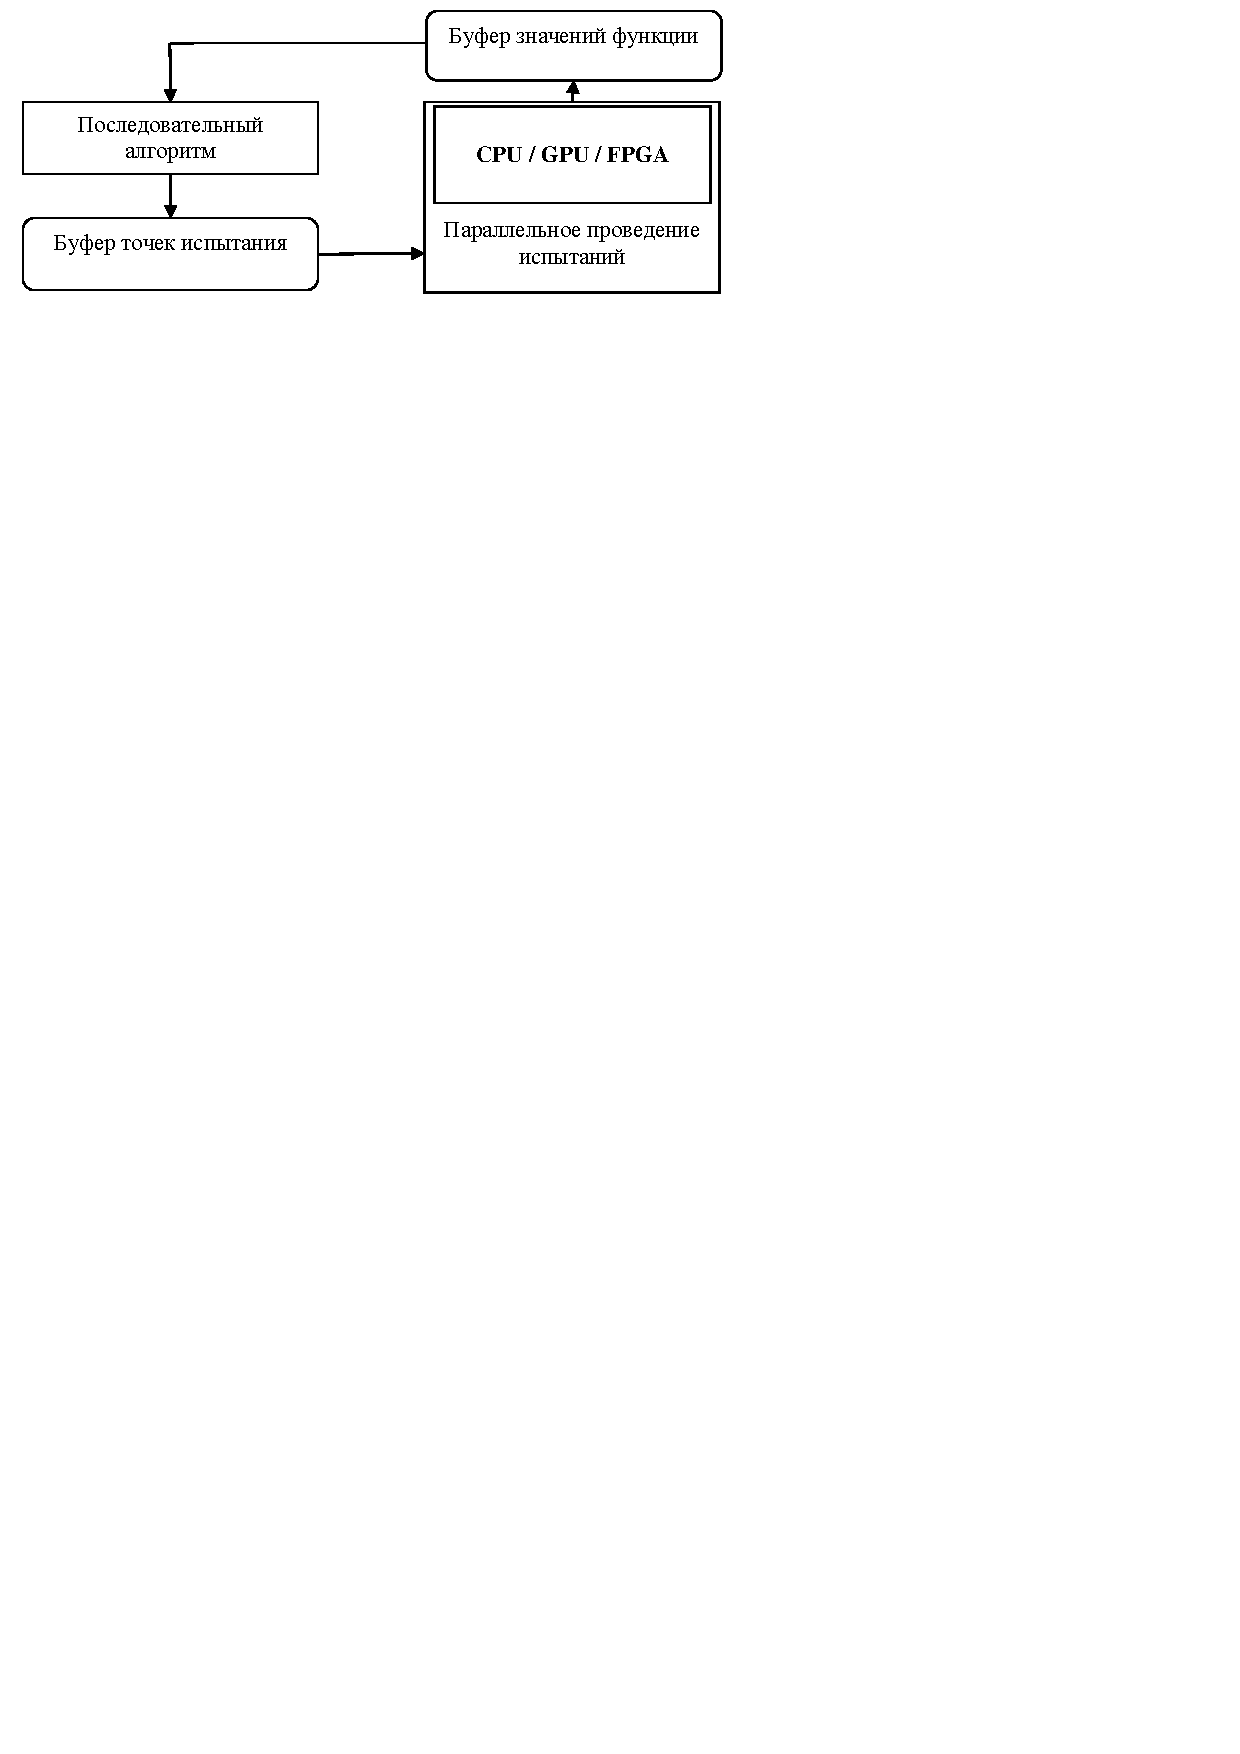
\includegraphics[width=0.7\linewidth]{./pic/s1.pdf}
  \bicaption{Общая схема организации параллельных вычислений.}{General scheme of organization of parallel computing.}
  \label{fig:s1}  
\end{center}
\end{figure}


\section{Результаты численных экспериментов}

Вычислительные эксперименты были проведены на компьютере с процессором Intel Core i5-10600 3.3GHz, 32 GB оперативной памяти и графической картой Intel UHD Graphics 630. Для получения исполняемого программного кода использовался компилятор Intel oneAPI DPC++ 2021.1.
Вычислительные эксперименты выполнялись с использованием  программной системы Globalizer [\ref{rfa:rulit:lit15}].

Большинство известных тестовых задач из области многомерной глобальной оптимизации характеризуются небольшим временем вычисления значений целевой функции, которое сопоставимо со временем работы расчетных правил алгоритма.
%Из-за этого при проведении экспериментов бывает сложно понять, с чем может быть связано относительно большое время выполнения параллельного алгоритма: с появившимися, сравнительно с последовательной версией, накладными расходами или причина в неэффективном распараллеливании. 
В прикладных оптимизационных задачах вычисление функции является трудоемкой операцией, здесь время работы алгоритма будет значительное меньше времени проведения одного испытания. 
В связи с этим нами была предложена модификация существующих тестовых задач, в которых требуется провести интегрирование исходной тестовой функции по части параметров. Для этого изначально порождается функция $\psi(y), y\in R^{2N},$ размерности $2N$, в которой первые $N$ координат фиксируются, а по остальным производится численное интегрирование по области определения функции. Для интегрирования используется метод средних прямоугольников. 

\begin{equation}
\varphi \left( {{y}_{1}},\ldots ,{{y}_{N}}~ \right)=\underset{{{a}_{N+1}}}{\overset{{{b}_{N+1}}}{\mathop \int }}\,\underset{{{a}_{N+2}}}{\overset{{{b}_{N+2}}}{\mathop \int }}\,\ldots \underset{{{a}_{2N}}}{\overset{{{b}_{2N}}}{\mathop \int }}\,\psi \left( {{y}_{1}},\ldots ,{{y}_{N}},{{y}_{N+1}},~..,{{y}_{2N}}~ \right)~d{{y}_{N+1}}d{{y}_{N+2}}..d{{y}_{2N}}~= 
\end{equation}
\begin{displaymath}
\underset{{{i}_{1}}=0}{\overset{M-1}{\mathop \sum }}\,\underset{{{i}_{2=0}}}{\overset{M-1}{\mathop \sum }}\,...\underset{{{i}_{N}}=0}{\overset{M-1}{\mathop \sum }}\,\left( \left( \underset{j=1}{\overset{2N}{\mathop \prod }}\,{{h}_{j}} \right)\psi \left( {{y}_{1}},{{y}_{2}},~..,{{y}_{N}},~{{y}_{{{\left( N+1 \right)}_{{{i}_{1}}}}}},{{y}_{{{\left( N+2 \right)}_{{{i}_{2}}}}}}~,~..,{{y}_{{{\left( 2N \right)}_{{{i}_{N}}}}}} \right) \right),
\end{displaymath}
\begin{displaymath}
D=\left\{ y~\in ~{{R}^{2N}}:~{{a}_{i}}\le {{y}_{i}}\le {{b}_{i}},~1\le i\le 2N \right\},
\end{displaymath}
\begin{equation}
{{y}_{{{\left( N+k \right)}_{{{i}_{k}}}}}}={{a}_{k}}+{{i}_{k}}{{h}_{k}}+\frac{{{h}_{k}}}{2},
\end{equation}
\begin{equation}
{{h}_{k}}=~\frac{{{b}_{k}}-~{{a}_{k}}}{M}.
\end{equation}
Здесь $M$ --- количество участков интегрирования по одной координате, а $\psi(y)$ --- исходная тестовая функция. Очевидно, чем больше значение $M$, тем больше проводится вычислений. Изменяя число узлов в сетке интегрирования по всем координатам или число участков по одной, можно регулировать время выполнения вычислений.


Вначале проведем вычислительные эксперименты с использованием классической тестовой функции Растригина
\begin{equation}
\label{Rastrigin}
\psi \left( {{y}_{1}},\ldots ,{{y}_{2N}}~ \right)=~\underset{i=1}{\overset{2N}{\mathop \sum }}\,(y_{i}^{2}-10\cos \left( 2\pi {{y}_{i}} \right)+10),
\end{equation}
\begin{displaymath}
-2.2<y\_i<1.8~,~1\le i\le 2N.
\end{displaymath}
На рис. \ref{fig:s2} изображены линии уровня двухмерной функции Растригина (слева) и модифицированной функции Растригина, в которой проводилось интегрирование по двум переменным (справа). Как можно видеть, новая функция не сильно отличается от исходной --- ее глобальный минимум остался прежним, в точке (0,0).

\begin{figure}
\begin{center}
  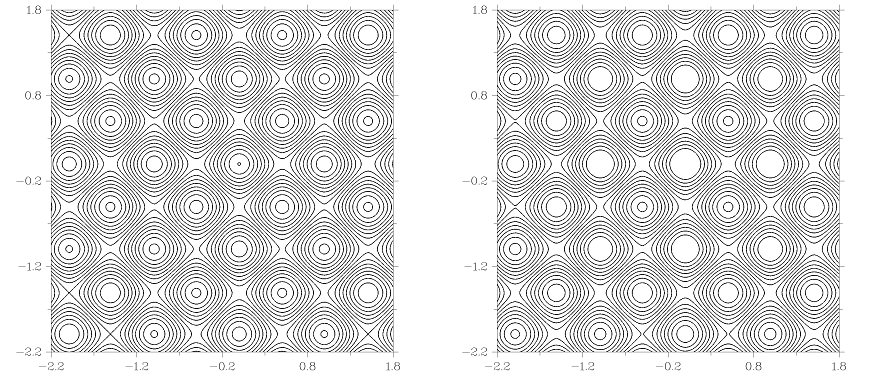
\includegraphics[width=1.0\linewidth]{./pic/s2.png}
  \bicaption{Линии уровня двумерной функции Растригина (слева) и модифицированной четырехмерной функции Растригина (справа).} {Level lines of the two-dimensional Rastrigin function (left) and the modified four-dimensional Rastrigin function (right).}
  \label{fig:s2}  
\end{center}
\end{figure}


При проведении экспериментов число испытаний параллельного алгоритма глобального поиска (ПАГП), было ограничено величиной $K_{max}=10^6$, точность поиска установлена $\varepsilon=0.01$, использовался параметр метода $r\ =\ 3$. Размерность решаемых задач была $N = 4$ и $N = 5$. При вычислениях на CPU число потоков варьировалось от 1 до 8, а при вычислении на GPU --- от 256 до 1024. Так как решались тестовые задачи, то использовался критерий остановки по попаданию в окрестность известного решения. В таблице \ref{table1} приведено число итераций ПАГП, в таблице \ref{table2} --- его ускорение по сравнению с однопоточным запуском.

\begin{table}[!ht]
    \centering
            \bicaption{Число итераций ПАГП при решении интегрированной функции Растригина.}{The number of iterations of PAGP when solving the integrated Rastrigin function.}
    \label{table1}
    \begin{tabular}{|l|l|l|l|l|l|l|l|l|}
    \hline
        N &\multicolumn{4}{c|}{CPU} & ~ & \multicolumn{3}{c|}{GPU} \\ \hline
        ~ & P=1 & P=2 & P=4 & P=8 &   & P=256 & P=512 & P=1024  \\ \hline
        4 & 61231 & 26592 & 21007 & 6728 &   & 340 & 301 & 92  \\ \hline
        5 & 703548 & 328141 & 258351 & 99524 &   & 4642 & 2194 & 995  \\ \hline
    \end{tabular}
\end{table}

\begin{table}[!ht]
    \centering
            \bicaption{Ускорение ПАГП при решении интегрированной функции Растригина} {Acceleration of GAGP in solving the integrated Rastrigin function}
    \label{table2}
    \begin{tabular}{|l|l|l|l|l|l|l|l|}
    \hline
        N &\multicolumn{3}{c|}{CPU} & ~ & \multicolumn{3}{c|}{GPU} \\ \hline
        ~ & P=2 & P=4 & P=8 & ~ & P=256 & P=512 & P=1024  \\ \hline
        4 & 2.1 & 2.1 & 5.6 & ~ & 2.8 & 3.1 & 9.4  \\ \hline
        5 & 1.9 & 2.0 & 4.3 & ~ & 2.4 & 4.9 & 9.7  \\ \hline
    \end{tabular}
\end{table}

Далее были проведены эксперименты на серии задач, полученных интегрированием функций из генератора GKLS. Данный генератор описан в [\ref{rfa:rulit:lit6}]. С его помощью можно порождать задачи многоэкстремальной оптимизации и варьировать их свойства: размерность, количество локальных минимумов, размеры их областей притяжения, координаты точки глобального минимума, значение функции в ней и т.д. На рис. \ref{fig:s3} изображены линии уровня двухмерной функции GKLS (слева) и модифицированной функции GKLS, полученной интегрированием четырехмерной функции по последним двум параметрам (справа).

\begin{figure}
\begin{center}
  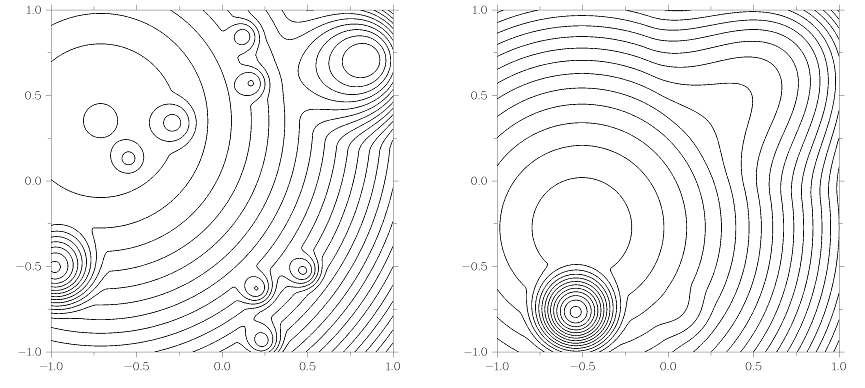
\includegraphics[width=1.0\linewidth]{./pic/s3.png}
  \bicaption{Функции GKLS (слева) и модифицированной функции GKLS (справа).}{GKLS function (left) and modified GKLS function (right).}
  \label{fig:s3}  
\end{center}
\end{figure}

Число итераций ПАГП было ограничено величиной $10^5$, точность поиска $\varepsilon=0.01$, параметр $r\ =\ 4$. Было сгенерировано две серии по 100 задач размерности $N = 4$ и $N = 5$. При вычислениях на CPU число потоков варьировалось от 1 до 8, а при вычислении на GPU от 256 до 1024. В таблице \ref{table3} приведено ускорение по сравнению с однопоточным запуском.

\begin{table}[!ht]
    \centering
    \bicaption{Ускорение ПАГП при решении серии модифицированных функций GKLS.}{Acceleration of GAGP when solving a series of modified GKLS functions.}
    \label{table3}
    \begin{tabular}{|l|l|l|l|l|l|l|l|}
    \hline
        N &\multicolumn{3}{c|}{CPU} & ~ & \multicolumn{3}{c|}{GPU} \\ \hline
        ~ & P=2 & P=4 & P=8 & ~ & P=256 & P=512 & P=1024  \\ \hline
        4 & 1.9 & 3.0 & 1.5 & ~ & 1.2 & 2.3 & 4.5  \\ \hline
        5 & 1.9 & 3.0 & 1.6 & ~ & 1.2 & 2.3 & 4.5  \\ \hline
    \end{tabular}
\end{table}

Полученные результаты подтверждают, что использование инструментов Intel oneAPI для реализации параллельного алгоритма глобального поиска позволяет написать одну версию кода, которая будет показывать хорошее ускорение как при использовании центрального процессора, так и при использовании графической карты. 



%=======================  Список литературы ==================================
%
% Команда \LITERRUS печатает "СПИСОК ЛИТЕРАТУРЫ" и обнуляет счетчики
%


\LITERRUS
% \rlitem{arg1}{arg2} --- создает пункт списка литературы.
% arg1 --- символическая ссылка на источник, используется при создании ссылки командой \ref
% arg2 --- текст, помещаемый в пункт списка. Может содержать команды выбора начертания 
%          символов и др.

\rlitem{rfa:rulit:lit1}{
\textit{Kutov D., Sulimov A., Sulimov V.} Supercomputer docking: investigation of low energy minima of protein-ligand complexes ~// Supercomputing Frontiers and Innovations, 2018. 5(3). 134--137. \doi{10.14529/jsfi180326}}

\rlitem{rfa:rulit:lit2}{
\textit{Абгарян К.К., Посыпкин М. А.} Применение оптимизационных методов для решения задач параметрической идентификации потенциалов межатомного взаимодействия ~// Ж. вычисл. матем. и матем. физ., 2014. \textbf{54}, N~12. 1994--2001. \doi{10.7868/S0044466914120023}}

\rlitem{rfa:rulit:lit3}{
\textit{Евтушенко Ю.Г., Лурье С.А., Посыпкин М.А., Соляев Ю.О.} Применение методов оптимизации для поиска равновесных состояний двумерных кристаллов ~// Ж. вычисл. матем. и матем. физ., 2016. \textbf{56}, N~12. 2032--2041. \doi{10.7868/S0044466916120097} }

\rlitem{rfa:rulit:lit4}{
\textit{Pinter J.D.} Global Optimization: Scientific and Engineering Case Studies. Springer, 2006.}

\rlitem{rfa:rulit:lit5}{
\textit{Gubaydullin I., Enikeeva L., Barkalov K., Lebedev I.} Parallel Global Search Algorithm for Optimization of the Kinetic Parameters of Chemical Reactions ~// Communications in Computer and Information Science, 2021. {\bf 1510}, 198--211. \doi{10.1007/978-3-030-92864-3_16}}

\rlitem{rfa:rulit:lit6}{
\textit{Сергеев, Я.Д., Квасов Д.Е.} Диагональные методы глобальной оптимизации. М.: Физматлит, 2008.}

\rlitem{rfa:rulit:lit8}{
\textit{Strongin R.G., Sergeyev Ya.D.} Global Optimization with Non-convex Constraints. Sequential and Parallel Algorithms. Kluwer Academic Publishers, 2000.}

\rlitem{rfa:rulit:lit9}{
\textit{Sergeyev Ya.D., Strongin R.G, Lera D.} Introduction to global optimization exploiting space-filling curves. Springer, 2013.}

\rlitem{rfa:rulit:lit10}{
\textit{Стронгин Р.Г., Гергель В.П., Гришагин В.А., Баркалов К.А.} Параллельные вычисления в задачах глобальной оптимизации. М.: Издательство Московского университета, 2013.}

\rlitem{rfa:rulit:lit11}{
\textit{Sovrasov V.} Comparison of several stochastic and deterministic derivative-free global optimization algorithms ~// Lecture Notes in Computer Science, 2019. \textbf{11548}. 70--81. \doi{10.1007/978-3-030-22629-9_6} }

\rlitem{rfa:rulit:lit12}{
\textit{Боресков А.А., Харламов А.А., Марковский Н.Д., Микушин Д.Н., Мортиков Е.В., Мыльцев А.А., Сахарных Н.А., Фролов В.А.} Параллельные вычисления на GPU. Архитектура и программная модель CUDA. М.:  Издательство Московского университета, 2015.}

\rlitem{rfa:rulit:lit13}{
\textit{Таненбаум Э., Остин Т.} Архитектура компьютера / перевод с английского Е. Матвеева. -- 6-е изд. Санкт-Петербург [и др.]: Питер, 2014.}

\rlitem{rfa:rulit:lit14}{
\textit{Комолов Д.А., Мяльк Р.А., Зобенко А.А., Филиппов А.С.} Системы автоматизированного проектирования фирмы Altera MAX+Plus II и Quartus II. Издательство РадиоСофт, 2002.}

\rlitem{rfa:rulit:lit15}{
\textit{Gergel V.P., Barkalov K.A., Sysoyev A.V.} A novel supercomputer software system for solving time-consuming global optimization problems ~// Numerical Algebra, Control and Optimization, 2018. \textbf{8}, N~1. 47--62. \doi{10.3934/naco.2018003}}


%\rlitem{rfa:rulit:lit7}{
%\textit{Paulavicius R., Zilinskas J, Grothey A.} Parallel branch and bound for global optimization with combination of Lipschitz bounds ~// Optimization Methods \& Software,  2011. \textbf{26}, N~3. 487--498. \doi{10.1080/10556788.2010.551537} }

%\rlitem{rfa:rulit:lit6__}{
%\textit{Захарова Е.М., Минашина И.К.} Обзор методов многомерной оптимизации. Информационные процессы, 2014. Т 14. №3. С. 256 -- 274.}

%\rlitem{rfa:rulit:lit9__}{
%\textit{Gablonsky J.M., Kelley C.T.} A Locally-Biased Form of the DIRECT Algorithm. Journal of Global Optimization, -- 2001, Vol. 21, No. 1, – P. 27--37.}


%\rlitem{rfa:rulit:lit95}{ %Эту ссылку можно убрать
%\textit{Sysoyev, A., Barkalov, K., Sovrasov, V., Lebedev, I., Gergel, V.} AGS NLP solver. \url{ https://github.com/sovrasov/ags_nlp_solver}}


%\rlitem{rfa:rulit:lit97}{
%\textit{Gaviano, M., Lera D., Kvasov D.E., Sergeyev Y.D.} Software for generation of classes of test functions with known local and global minima for global optimization/ M. Gaviano, D. Lera, D. E. Kvasov, Y. D. Sergeyev // ACM Transactions on Mathematical Software, 2003. Vol. 29. P. 469-480.}

%=======================  Список литературы ==================================
\medskip
\DateRU 

\medskip

\MakeAuthorsInfoRU

%===========================  REFERENCES =====================================
\pagebreak

\REFERENCES

\elitem{rfa:enlit:lit1}{
\textit{D. Kutov, A. Sulimov, V. Sulimov} ``Supercomputer docking: investigation of low energy minima of protein-ligand complexes,'' Supercomputing Frontiers and Innovations. 5(3), 134--137 (2018). \doi{10.14529/jsfi180326}}

\elitem{rfa:enlit:lit2}{
\textit{K.K. Abgaryan, M.A. Posypkin } ``Application of optimization methods for solving problems of parametric identification of interatomic interaction potentials,'' Comput. Math. Math. Phys. 54(12), 1994--2001 (2014). [in Russian] \doi{10.7868/S0044466914120023}}

\elitem{rfa:enlit:lit3}{
\textit{Yu.G. Yevtushenko, S.A. Lurie, M.A. Posypkin, Y.O. Solyaev } ``Application of optimization methods for finding equilibrium states of two-dimensional crystals,'' Comput. Math. Math. Phys. 56(12), 2032--2041 (2016). [in Russian] \doi{10.7868/S0044466916120097}}

\elitem{rfa:enlit:lit4}{
\textit{J.D. Pinter} Global Optimization: Scientific and Engineering Case Studies. Springer, 2006.}

\elitem{rfa:enlit:lit5}{
\textit{I. Gubaydullin, L. Enikeeva, K. Barkalov, I. Lebedev} ``Parallel Global Search Algorithm for Optimization of the Kinetic Parameters of Chemical Reactions,'' Communications in Computer and Information Science. 1510, 198--211 (2021). \doi{10.1007/978-3-030-92864-3_16}}

\elitem{rfa:enlit:lit6}{
\textit{Ya.D. Sergeev, D.E. Kvasov } Diagonal Global Optimization Methods  (Fizmatlit, Moscow, 2008) [in Russian]}

\elitem{rfa:enlit:lit8}{
\textit{R.G. Strongin, Ya.D. Sergeyev } Global Optimization with Non-convex Constraints. Sequential and Parallel Algorithms. Kluwer Academic Publishers, 2000.}

\elitem{rfa:enlit:lit9}{
\textit{Ya.D. Sergeyev,  R.G. Strongin, D. Lera } Introduction to global optimization exploiting space-filling curves. Springer, 2013.}

\elitem{rfa:enlit:lit10}{
\textit{R.G. Strongin, V.P. Gergel, V.A. Grishagin, K.A. Barkalov } Parallel Computations in Global Optimization Problems (Izd. Mosk.
Gos. Univ., Moscow, 2013.) [in Russian]}

\elitem{rfa:enlit:lit11}{
\textit{V. Sovrasov } ``Comparison of several stochastic and deterministic derivative-free global optimization algorithms,'' Lecture Notes in Computer Science. 11548, 70--81 (2019). \doi{10.1007/978-3-030-22629-9_6}}

\elitem{rfa:enlit:lit12}{
\textit{A.A. Boreskov, A.A. Kharlamov, N.D. Markovsky, D.N. Mikushin, E.V. Mortikov, A.A. Myltsev, N.A. Sakharnykh, V.A. Frolov } Parallel computing on the GPU. Architecture and programming model of CUDA. (Izd. Mosk. Gos. Univ., Moscow, 2015.) [in Russian]}

\elitem{rfa:enlit:lit13}{
\textit{A. Tanenbaum, T. Austin} Structured Computer Organization / translation from English by E. Matveeva. -- 6th ed. ( Piter, Saint Petersburg, 2014.) [in Russian]}

\elitem{rfa:enlit:lit14}{
\textit{D.A. Komolov, R.A. Myalk, A.A. Zobenko, A.S. Filippov} Computer-aided design systems from Altera MAX+Plus II and Quartus II. ( RadioSoft Publishing House, Moscow, 2002.) [in Russian]}

\elitem{rfa:enlit:lit15}{
\textit{ V.P. Gergel, K.A. Barkalov, A.V. Sysoyev} ``A novel supercomputer software system for solving time-consuming global optimization problems,'' Numerical Algebra, Control and Optimization. 8(1), 47--62 (2018). \doi{10.3934/naco.2018003}}


%\elitem{rfa:enlit:lit7}{
%\textit{R. Paulavicius, J. Zilinskas, A. Grothey } ``Parallel branch and bound for global optimization with combination of Lipschitz bounds,'' Optimization Methods \& Software. 26(3), 487--498 (2011). \doi{10.1080/10556788.2010.551537} }

\medskip
\DateEN

\bigskip

\MakeAuthorsInfoEN

%\end{document}
%============================ КОНЕЦ СТАТЬИ ==================================




\end{document}

